%package list
\documentclass{article}
\usepackage[top=3cm, bottom=3cm, outer=3cm, inner=3cm]{geometry}
\usepackage{multicol}
\usepackage{graphicx}
\usepackage{url}
%\usepackage{cite}
\usepackage{hyperref}
\usepackage{array}
%\usepackage{multicol}
\newcolumntype{x}[1]{>{\centering\arraybackslash\hspace{0pt}}p{#1}}
\usepackage{natbib}
\usepackage{pdfpages}
\usepackage{multirow}
\usepackage[normalem]{ulem}
\useunder{\uline}{\ul}{}
\usepackage{svg}
\usepackage{xcolor}
\usepackage{listings}

\lstdefinestyle{ascii-tree}{
    literate={├}{|}1 {─}{--}1 {└}{+}1 
  }
\lstset{basicstyle=\ttfamily,
  showstringspaces=false,
  commentstyle=\color{red},
  keywordstyle=\color{blue}
}
%\usepackage{booktabs}
\usepackage{caption}
\usepackage{subcaption}
\usepackage{float}
\usepackage{array}

\newcolumntype{M}[1]{>{\centering\arraybackslash}m{#1}}
\newcolumntype{N}{@{}m{0pt}@{}}


%%%%%%%%%%%%%%%%%%%%%%%%%%%%%%%%%%%%%%%%%%%%%%%%%%%%%%%%%%%%%%%%%%%%%%%%%%%%
%%%%%%%%%%%%%%%%%%%%%%%%%%%%%%%%%%%%%%%%%%%%%%%%%%%%%%%%%%%%%%%%%%%%%%%%%%%%
\newcommand{\itemEmail}{kllacma@unsa.edu.pe}
\newcommand{\itemStudent}{Kevin Andree Llacma Quispe}
\newcommand{\itemCourse}{Programacion web 2}
\newcommand{\itemCourseCode}{20200585}
\newcommand{\itemSemester}{I}
\newcommand{\itemUniversity}{Universidad Nacional de San Agustín de Arequipa}
\newcommand{\itemFaculty}{Facultad de Ingeniería de Producción y Servicios}
\newcommand{\itemDepartment}{Departamento Académico de Ingeniería de Sistemas e Informática}
\newcommand{\itemSchool}{Escuela Profesional de Ingeniería de Sistemas}
\newcommand{\itemAcademic}{2024 - A}
\newcommand{\itemInput}{-}
\newcommand{\itemOutput}{-}
\newcommand{\itemPracticeNumber}{04}
\newcommand{\itemTheme}{python}
%%%%%%%%%%%%%%%%%%%%%%%%%%%%%%%%%%%%%%%%%%%%%%%%%%%%%%%%%%%%%%%%%%%%%%%%%%%%
%%%%%%%%%%%%%%%%%%%%%%%%%%%%%%%%%%%%%%%%%%%%%%%%%%%%%%%%%%%%%%%%%%%%%%%%%%%%

\usepackage[english,spanish]{babel}
\usepackage[utf8]{inputenc}
\AtBeginDocument{\selectlanguage{spanish}}
\renewcommand{\figurename}{Figura}
\renewcommand{\refname}{Referencias}
\renewcommand{\tablename}{Tabla} %esto no funciona cuando se usa babel
\AtBeginDocument{%
	\renewcommand\tablename{Tabla}
}

\usepackage{fancyhdr}
\pagestyle{fancy}
\fancyhf{}
\setlength{\headheight}{30pt}
\renewcommand{\headrulewidth}{1pt}
\renewcommand{\footrulewidth}{1pt}
\fancyhead[L]{\raisebox{-0.2\height}{
\includegraphics[width=3cm]{img/logo_episunsa.png}}}
\fancyhead[C]{\fontsize{7}{7}\selectfont	\itemUniversity \\ \itemFaculty \\ \itemDepartment \\ \itemSchool \\ \textbf{\itemCourse}}
\fancyhead[R]{\raisebox{-0.2\height}{
\includegraphics[width=1.2cm]{img/logo_abet}}}
\fancyfoot[L]{Estudiante Kevin Llacma}
\fancyfoot[C]{\itemCourse}
\fancyfoot[R]{Página \thepage}

% para el codigo fuente

\usepackage{listings}
\usepackage{color, colortbl}
\definecolor{dkgreen}{rgb}{0,0.6,0}
\definecolor{gray}{rgb}{0.5,0.5,0.5}
\definecolor{mauve}{rgb}{0.58,0,0.82}
\definecolor{codebackground}{rgb}{0.95, 0.95, 0.92}
\definecolor{tablebackground}{rgb}{0.8, 0, 0}

\lstset{frame=tb,
	language=bash,
	aboveskip=3mm,
	belowskip=3mm,
	showstringspaces=false,
	columns=flexible,
	basicstyle={\small\ttfamily},
	numbers=none,
	numberstyle=\tiny\color{gray},
	keywordstyle=\color{blue},
	commentstyle=\color{dkgreen},
	stringstyle=\color{mauve},
	breaklines=true,
	breakatwhitespace=true,
	tabsize=3,
	backgroundcolor= \color{codebackground},
}

\begin{document}
	
	\vspace*{10px}
	
	\begin{center}	
		\fontsize{17}{17} \textbf{ Informe de Laboratorio \itemPracticeNumber}
	\end{center}
	\centerline{\textbf{\Large Tema: \itemTheme}}
	%\vspace*{0.5cm}	

	\begin{flushright}
		\begin{tabular}{|M{2.5cm}|N|}
			\hline 
			\rowcolor{tablebackground}
			\color{white} \textbf{Nota}  \\
			\hline 
			     \\[30pt]
			\hline 			
		\end{tabular}
	\end{flushright}	

	\begin{table}[H]
		\begin{tabular}{|x{4.7cm}|x{4.8cm}|x{4.8cm}|}
			\hline 
			\rowcolor{tablebackground}
			\color{white} \textbf{Estudiante} & \color{white}\textbf{Escuela}  & \color{white}\textbf{Asignatura}   \\
			\hline 
			{\itemStudent \par \itemEmail} & \itemSchool & {\itemCourse \par Semestre: \itemSemester \par Código: \itemCourseCode}     \\
			\hline 			
		\end{tabular}
	\end{table}		
	
	\begin{table}[H]
		\begin{tabular}{|x{4.7cm}|x{4.8cm}|x{4.8cm}|}
			\hline 
			\rowcolor{tablebackground}
			\color{white}\textbf{Laboratorio} & \color{white}\textbf{Tema}  & \color{white}\textbf{Duración}   \\
			\hline 
			\itemPracticeNumber & \itemTheme & 04 horas   \\
			\hline 
		\end{tabular}
	\end{table}
	
	\begin{table}[H]
		\begin{tabular}{|x{4.7cm}|x{4.8cm}|x{4.8cm}|}
			\hline 
			\rowcolor{tablebackground}
			\color{white}\textbf{Semestre académico} & \color{white}\textbf{Fecha de inicio}  & \color{white}\textbf{Fecha de entrega}   \\
			\hline 
			\itemAcademic & \itemInput &  \itemOutput  \\
			\hline 
		\end{tabular}
	\end{table}
\title{Programación Web\\Laboratorio 05\\Tema: python}

\maketitle


\section{Competencias}




    \begin{itemize}
        \item General: C.c. Diseña responsablemente aplicaciones web, sus componentes o procesos para satisfacer necesidades dentro de restricciones realistas: económicas, medio ambientales, sociales,políticas, éticas, de salud, de seguridad, manufacturación y sostenibilidad.
        \item Específica: C.m. Construye responsablemente soluciones con tecnología web siguiendo un proceso adecuado llevando a cabo las pruebas ajustada a los recursos disponibles del cliente.
        \item Específica: C.p. Aplica de forma flexible técnicas, métodos, principios, normas, estándares y herramientas del desarrollo web necesarias para la construcción de aplicaciones web e implementación de estos sistemas en una organización.
        
    \end{itemize}


\section{Desarollo del lab}
\subsection{Descripcion}
\textbf{Ejercicio2a }
\\para realziar el ejercicio se tuvo que modificar el archivo picture.py

\\.Usando los metodos negative, join y up


    \begin{figure}[H]
		          \centering
		          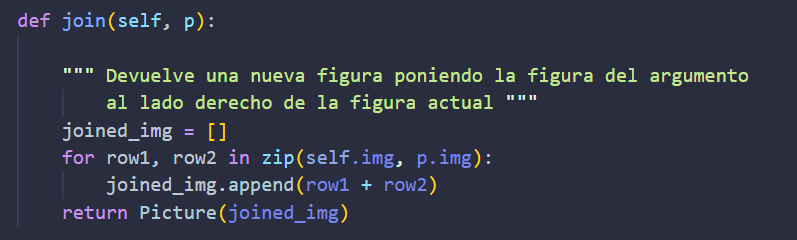
\includegraphics[width=0.8\textwidth,keepaspectratio]                       {img/picJoin.png}
		             %\includesvg{img/automata.svg}
		              %\label{img:mot2}
		              %\caption{Product backlog.}
    \end{figure}
\\
    \begin{figure}[H]
		          \centering
		          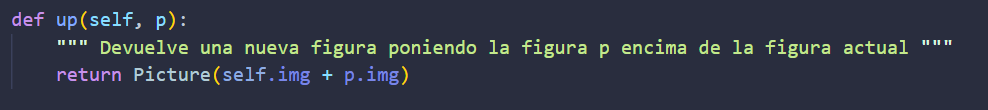
\includegraphics[width=0.8\textwidth,keepaspectratio]                       {img/picUp.png}
		             %\includesvg{img/automata.svg}
		              %\label{img:mot2}
		              %\caption{Product backlog.}
    \end{figure}

\\    
 \begin{figure}[H]
		          \centering
		          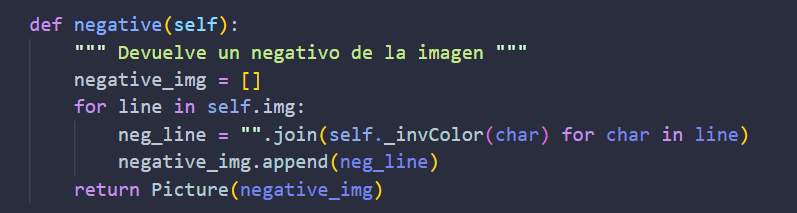
\includegraphics[width=0.8\textwidth,keepaspectratio]                       {img/picNeg.png}
		             %\includesvg{img/automata.svg}
		              %\label{img:mot2}
		              %\caption{Product backlog.}
    \end{figure}

\\    
Primero crea los caballos blanco y negro que seria negativo. Luego
une horizontalmente el caballo blanco (knight white) y el caballo negro invertido (knight black). despues a lo contrario
Finalemnte los une 
    \begin{figure}[H]
		          \centering
		          \includegraphics[width=0.8\textwidth,keepaspectratio]                       {img/eja.png}
		             %\includesvg{img/automata.svg}
		              %\label{img:mot2}
		              %\caption{Product backlog.}
    \end{figure}
\\
\textbf{Ejercicio2b }
Para este ejercicio. Se uso lo mismo que en anterior cambiando por vertical mirror los dos de abajo


     \begin{figure}[H]
		          \centering
		          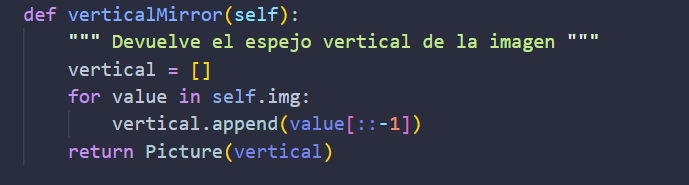
\includegraphics[width=0.8\textwidth,keepaspectratio]                       {img/picVerm.png}
		             %\includesvg{img/automata.svg}
		              %\label{img:mot2}
		              %\caption{Product backlog.}
    \end{figure}
\\
\\Podemos observar que lo hacemos para que los caballos de abajo miren al contrario
    \begin{figure}[H]
		          \centering
		          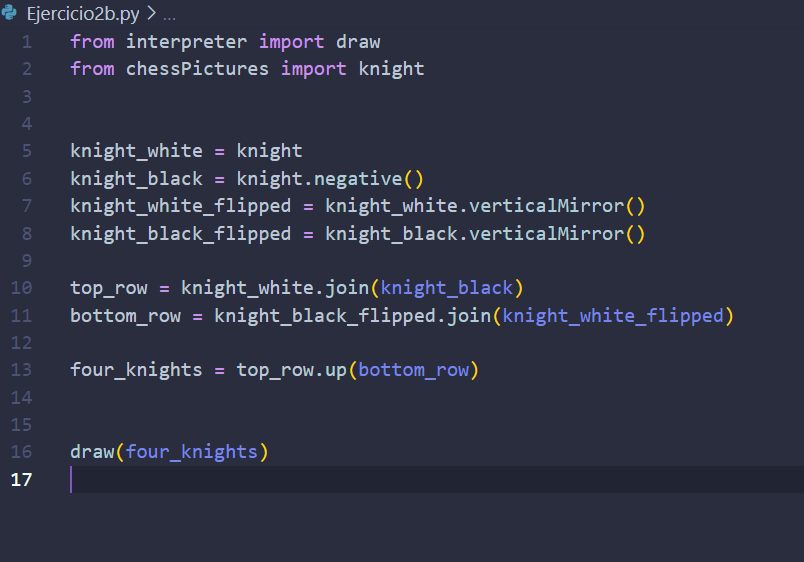
\includegraphics[width=0.8\textwidth,keepaspectratio]                       {img/Ejb.png}
		             %\includesvg{img/automata.svg}
		              %\label{img:mot2}
		              %\caption{Product backlog.}
    \end{figure}
\
\textbf{Ejercicio2c }
\\Para este ejercicio se hace uso de horizontalRepeat:
\begin{itemize}
    \item Toma la imagen actual (self.img), la expande horizontalmente n veces y devuelve esta nueva imagen como una instancia de la clase Picture.
    \item Cada fila de la imagen original se concatena n veces para formar la nueva imagen expandida horizontalmente.
\end{itemize}

    \begin{figure}[H]
		          \centering
		          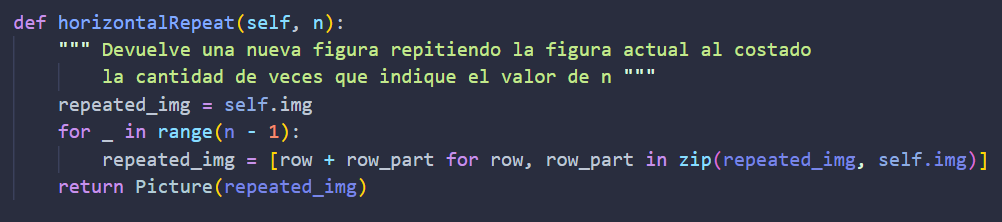
\includegraphics[width=0.8\textwidth,keepaspectratio]                       {img/picHor.png}
		             %\includesvg{img/automata.svg}
		              %\label{img:mot2}
		              %\caption{Product backlog.}
    \end{figure}
\\lLe mandamos para que repita 4 veces la misma imagen

    \begin{figure}[H]
		          \centering
		          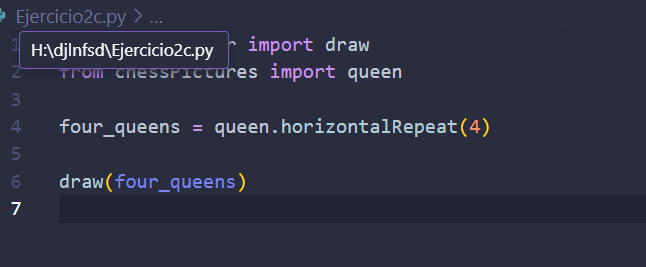
\includegraphics[width=0.8\textwidth,keepaspectratio]                       {img/Ejc.png}
		             %\includesvg{img/automata.svg}
		              %\label{img:mot2}
		              %\caption{Product backlog.}
    \end{figure}


\textbf{Ejercicio2d }
\\Combinamos lo que habuiamos hecho usando horizontalrepeat y join para imprimir cuadrados intercalando color y haciendolo horizontalmente

     \begin{figure}[H]
		          \centering
		          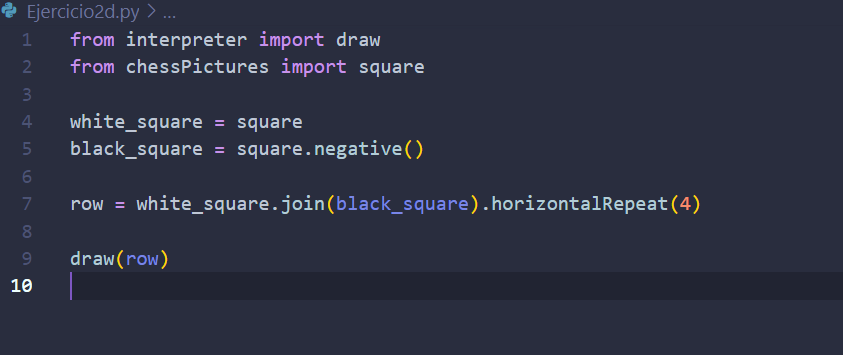
\includegraphics[width=0.8\textwidth,keepaspectratio]                       {img/Ejd.png}
		             %\includesvg{img/automata.svg}
		              %\label{img:mot2}
		              %\caption{Product backlog.}
    \end{figure}

\textbf{Ejercicio2e }
\\Lo mismo solo que ahora empieza con el color contario

     \begin{figure}[H]
		          \centering
		          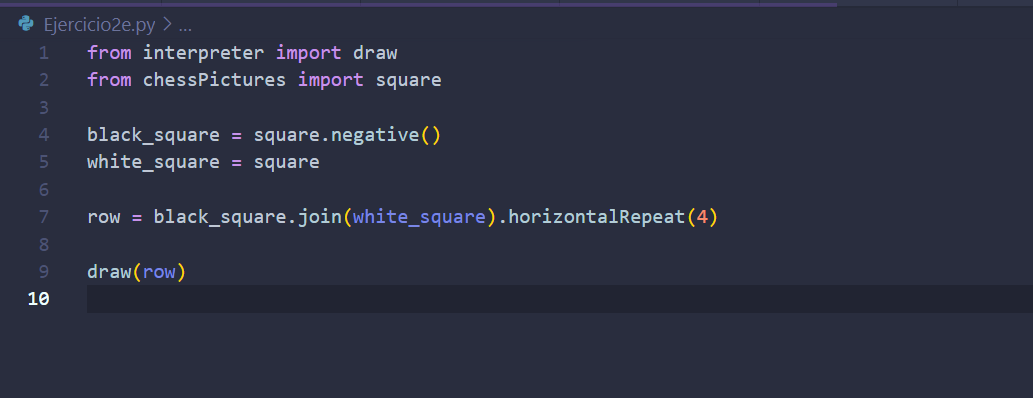
\includegraphics[width=0.8\textwidth,keepaspectratio]                       {img/Eje.png}
		             %\includesvg{img/automata.svg}
		              %\label{img:mot2}
		              %\caption{Product backlog.}
    \end{figure}
\textbf{Ejercicio2f }
\\Ahora hacemos uso de un nuevo metodo verticalrepeat

    \begin{figure}[H]
		          \centering
		          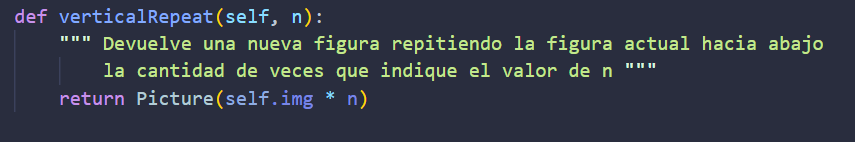
\includegraphics[width=0.8\textwidth,keepaspectratio]                       {img/picVer.png}
		             %\includesvg{img/automata.svg}
		              %\label{img:mot2}
		              %\caption{Product backlog.}
    \end{figure}
    
\\Ahora agregamos el metodo join para imprimir mas de 2 filas. Creamos 2 filas una empieza con blanco y la optra con negro y se unen. Finalmente se repiten 2 veces hacia abajo

    \begin{figure}[H]
		          \centering
		          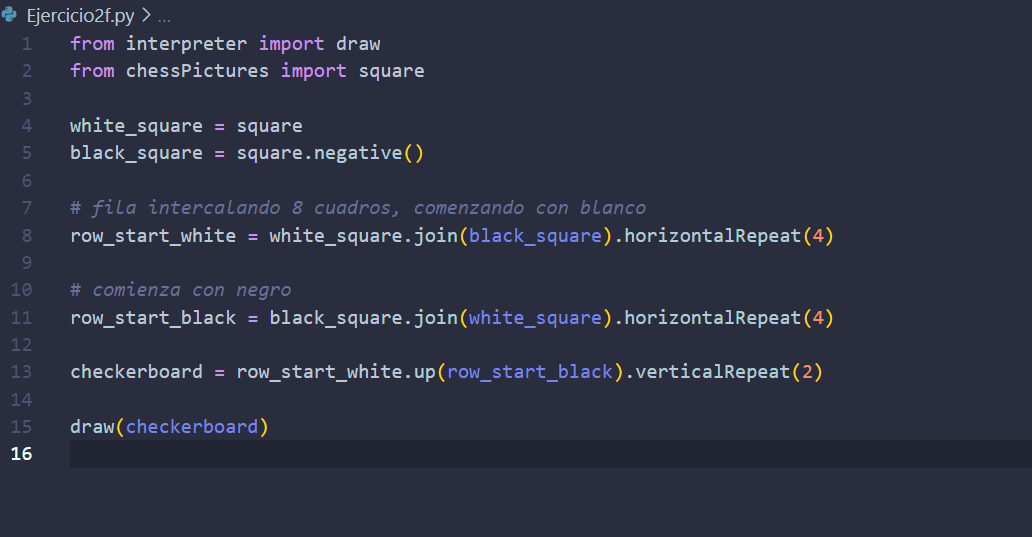
\includegraphics[width=0.8\textwidth,keepaspectratio]                       {img/Ejef.png}
		             %\includesvg{img/automata.svg}
		              %\label{img:mot2}
		              %\caption{Product backlog.}
    \end{figure}

\\
\textbf{Ejercicio2g }
\\Hacemos uso de los que implementamos anterioremente

    \begin{figure}[H]
		          \centering
		          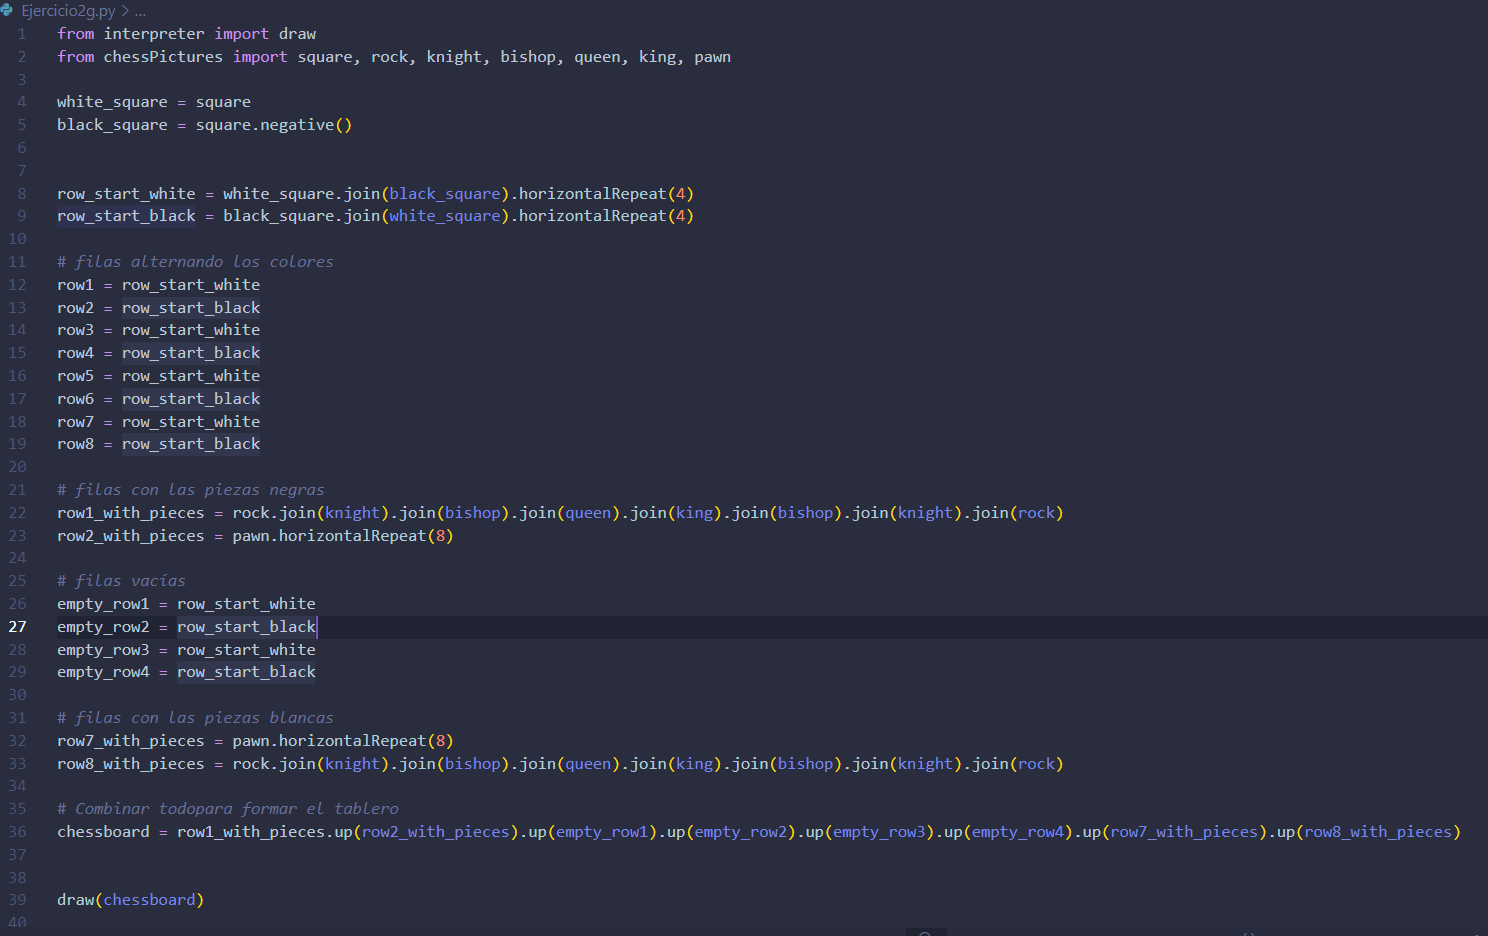
\includegraphics[width=0.8\textwidth,keepaspectratio]                       {img/Ejg.png}
		             %\includesvg{img/automata.svg}
		              %\label{img:mot2}
		              %\caption{Product backlog.}
    \end{figure}    
\\


\end{document}